
Introducción al capítulo

\section{Descripción de los servicios web - necesarios}
\section{Modelo de datos}

Debe explicar el modelo de datos, relacional o no-relacional, es decir leerlo destacando las entidades, colecciones y/o relaciones -referencias fundamentales en la problemática.
Diagrama con Modelo de datos relacional o no relacional

\begin{figure}[H]
    \centering
    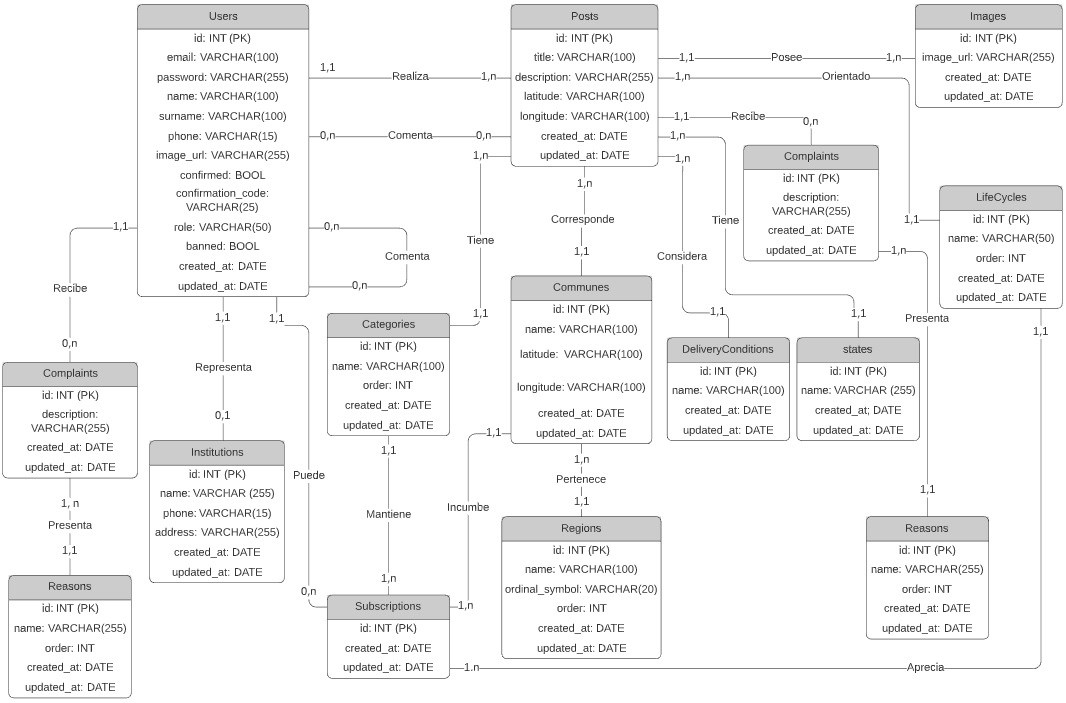
\includegraphics[scale=0.5]{figures/i4.jpg}
    \caption{XX}
    \label{fig:i4}
\end{figure}

\begin{figure}[H]
    \centering
    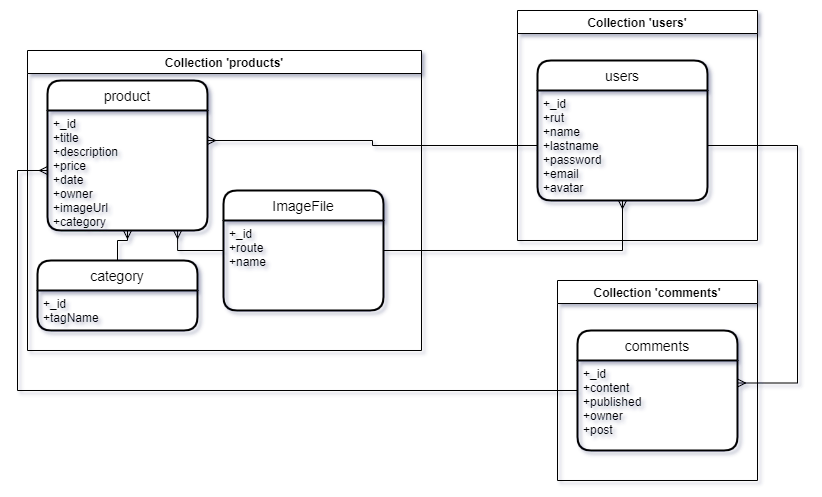
\includegraphics[scale=0.5]{figures/i5.png}
    \caption{xx}
    \label{fig:i5}
\end{figure}

\subsection{Esquema de la base de datos}

A continuación, se describen los datos y tipos de la BD, en formato JSON.

Esquema products : 

% Se dejo en comentarios, porque depende de lo que hagan
%{
%    title: {
%        type: String,
%        required: true
%    },
%    description: {
%        type: String,
%        default: null
%    },
%    price: {
%        type: Number,
%        required: true
%    },
%    date: {
%        type: Date,
%        required: true
%    },
%    imageUrl: [{
%        type: Schema.ObjectId,
%        ref: "imageFile"
%    }],
%    owner: {
%        type: Schema.ObjectId,
%        ref: "user"
%    },
%    category: [{
%        type: Schema.ObjectId,
%        ref: "category"
%    }],
%}

\subsection{Entidad-Relación}
\subsection{Modelo Relacional}


\section{Casos de uso (o Historias de usuario)}
\subsection{Actores de casos de uso}

Los actores que interactúan con el sistema se detallan en la Tabla 13.

\begin{table}[H]
    \begin{center}
        \begin{tabular}{ |m{2cm}|m{2cm}|m{3cm}|m{3cm}|m{3cm}| }
            \hline 
            \textbf{Actor} & \textbf{Cargo(s)} & \textbf{Funciones en la empresa} &
            \textbf{Nivel de conocimeintos técnicos requeridos} & \textbf{Nivel privilegio en el sistema} \\ \hline
              &   &   &   &  \\ \hline
              &   &   &   &  \\ \hline
        \end{tabular}
        \caption{ Calculo costo de desarrollo y soporte.}
    \end{center}
\end{table}

En el caso de que existen generalizaciones de actores incluya los diagramas correspondientes.

\subsection{Diagramas}

Incluya más de 1 diagrama para que quede claro el modelo.
Diagrama(s) de CU


\begin{figure}[H]
    \centering
    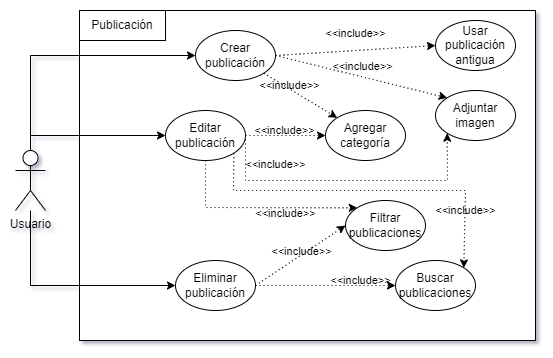
\includegraphics[scale=0.5]{figures/i3.png}
    \caption{Diagrama de Casos de Uso publicaciones – ejemplo tesis Tomás Montecinos IECI}
    \label{fig:e3}
\end{figure}

\subsection{Especificación de casos de uso}

Liste los CU que están en su (s) diagramas destacando cuales serán detallados.
Considerando funcionalidad RELEVANTE del negocio especifique con la tabla sólo los CU relacionados. Para los CU restantes sólo incluya una descripción y precondiciones.


\begin{figure}[H]
    \centering
    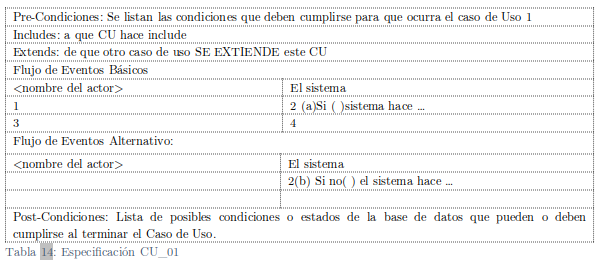
\includegraphics[scale=0.5]{figures/i12.png}
    \caption{E1}
    \label{fig:i12}
\end{figure}

Ejemplos:

\begin{figure}[H]
    \centering
    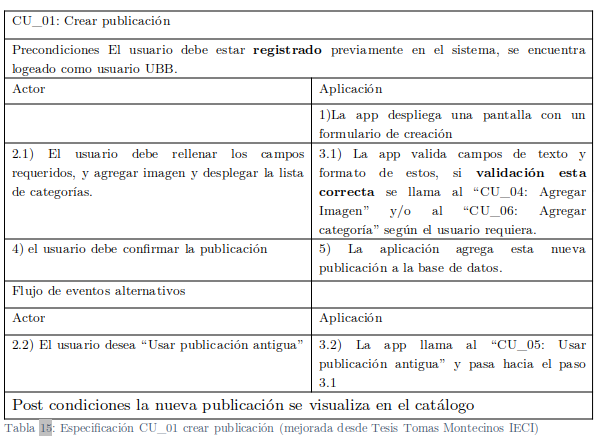
\includegraphics[scale=0.5]{figures/i13.png}
    \caption{E2}
    \label{fig:i13}
\end{figure}



\section{Diseño de interfaz y navegación (Mockups)}

\subsection{Guías de estilos}

La guía de estilo marcará las pautas a seguir para el diseño de la web. Por tanto, servirá
de consulta para visualizar los objetivos de la aplicación en cuanto a su estilo. El principal
objetivo es dotar al estilo de la aplicación de la máxima sencillez posible, a fin de que al
usuario le resulte intuitivo el uso de la aplicación.
A continuación se señalarán aspectos relativos al estilo como son el logotipo, los colores
principales y secundarios, la tipografía y la composición de las interfaces.
\subsubsection{Logotipo}
El logotipo es el símbolo que representa la temática de la aplicación. Esta imagen podrá ser presentada de diferentes formas, como son el imagotipo y el isotipo. Además, se mostrarán dos versiones de cada representación: una en color y otra en blanco y negro.
Por lo que respecta al isotipo, en la figura 8.8, este se caracteriza por no tener ningún texto. El icono representativo se caracteriza por estar compuesto por dos elementos. El principal es un coche con 5 pasajeros, simbolizando el hecho de compartir coche, mientras que el secundario se trata del icono representativo de la ubicación con un birrete, que simboliza el hecho de encontrar estudiantes.

\begin{figure}[H]
    \centering
    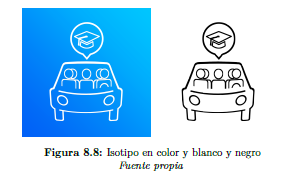
\includegraphics[scale=0.5]{figures/i11.png}
    \caption{autitos}
    \label{fig:i11}
\end{figure}

\subsection{Guía de colores}

Los colores corporativos de la aplicación componen una gama cromática fría, orientada a
tonos azules. En primer lugar, los colores corporativos que se utilizarán mayoritariamente en el diseño de las interfaces están reunidos en la paleta de la figura 8.10. Por una parte, “Bluetiful” y “Vivid Sky Blue” serán los colores de los elementos con los que el usuario podrá interactuar, como botones y enlaces. Y, por otra parte, “Black Chocolate” y “Azyre X Web Color” serán los correspondientes al texto y fondo de la aplicación

\begin{figure}[H]
    \centering
    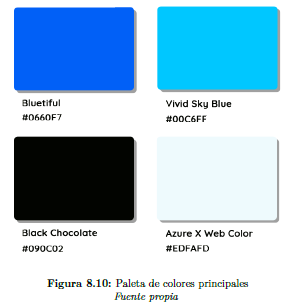
\includegraphics[scale=0.5]{figures/i9.png}
    \caption{autitos}
    \label{fig:i9}
\end{figure}

No obstante, a estos colores principales se les añadirán 3 más que estarán relacionados con la acción que realizan los botones en los que se apliquen. Se trata del color “Rufous” para acciones como “Eliminar” y “Cancelar”, el “Maximum Yellow” para “Editar” y “Leaf Green” para “Enviar” y “Aceptar”.

\begin{figure}[H]
    \centering
    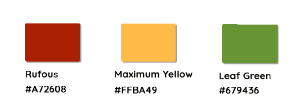
\includegraphics[scale=0.5]{figures/i8.png}
    \caption{autitos}
    \label{fig:i8}
\end{figure}

\subsubsection{Tipografía}

La tipografía utilizada es un tipo de letra sencilla y universal que facilite la legibilidad. Se ha optado por emplear una fuente gratuita de Google Fonts, como es Roboto. En la figura se incluye una representación de dicha fuente con los caracteres más comunes.

\begin{figure}[H]
    \centering
    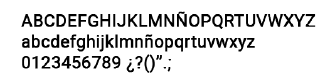
\includegraphics[scale=0.5]{figures/i10.png}
    \caption{autitos}
    \label{fig:i10}
\end{figure}

\subsection{Composición de las interfaces}

La composición de las interfaces expuesta a continuación corresponde a la versión adaptada para móvil, que será la versión implementada en primer lugar. La adaptación para pantallas de mayor tamaño se realizará en un futuro.
Distinguiremos entre 3 tipos de interfaces según su composición: lista, tarjeta y formulario. La comparación entre ellas puede observarse en la figura 

\begin{figure}[H]
    \centering
    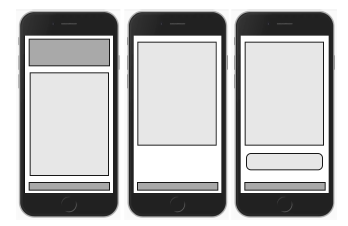
\includegraphics[scale=0.5]{figures/i7.png}
    \caption{autitos}
    \label{fig:i7}
\end{figure}

<Incluye al menos 3 mockups o screenshot de las interfaces propuestas que representan el estándar que será seguido en el sw>.

Recuerde: El diseño de la interfaz de usuario debe considerar un diseño estándar que será respetado en todas las pantallas. En el diseño se considera la organización y el aspecto de la interfaz. El aspecto considera muchos elementos, entre ellos, los colores, imágenes de fondo, uso de iconos entre otros. La organización de una pantalla considera la ubicación de cada uno de los tipos de elementos de la interfaz, considerando por ejemplo las siguientes áreas:  De ingresos de datos, De Botones de opción general, De botones de opciones específicas a la ventana, De Menús, De títulos,  De Barras de Herramientas, De pie de página, De Encabezados, y De Logos
